\documentclass[11pt,a4paper]{article}

\usepackage[utf8]{inputenc}
\usepackage[T1]{fontenc}
\usepackage{lmodern}
\usepackage[margin=2.3cm]{geometry}
\usepackage{graphicx}
\usepackage{booktabs}
\usepackage{multirow}
\usepackage{amsmath}
\usepackage{xcolor}
\usepackage[font=small,labelfont=bf]{caption}
\usepackage{subcaption}
\usepackage[numbers,sort&compress]{natbib}
\usepackage[hidelinks]{hyperref}
\usepackage{enumitem}
\usepackage{microtype}
\emergencystretch=1.5em
\setlist{nosep,leftmargin=*}

\graphicspath{{../figures/}}
\newcommand{\todo}[1]{\textcolor{red}{[TODO: #1]}}
\newcommand{\code}[1]{\texttt{#1}}

\title{Predicting the Quality of Experience of Mobile Video Sessions\\
       on the PoQeMoN Dataset}
\author{Gonzalo \todo{surname} \and Salma \todo{surname}}
\date{CSC~7018 Data Science: Theory to Practice --- Télécom SudParis\\[2pt]
      November 2026\\[8pt]
      \small Code: \url{https://github.com/Notwegiangir/qoe-poqemon-project}}

\begin{document}

\hypersetup{pageanchor=false}
\begin{titlepage}
  \maketitle
  \thispagestyle{empty}
  \begin{abstract}
    \noindent We predict the Mean Opinion Score (MOS, 1--5) of mobile YouTube sessions from the
    QoE influence factors of the PoQeMoN dataset (1{,}543 sessions, 181 testers). Five classifiers
    (a majority-class baseline, $k$-nearest neighbours, SVC, decision tree and XGBoost) are tuned by
    grid search with user-grouped cross-validation and evaluated once on held-out users. We compare two
    feature sets: \emph{objective} factors that can be measured without asking the user
    (player, network, device and user profile), and the same factors \emph{with} the testers' own
    feedback ratings. With feedback, XGBoost reaches a test macro-F1 of 0.689 (accuracy 0.753, MAE 0.27 MOS
    points). Without feedback, the best model reaches only 0.41--0.45 macro-F1 (accuracy 0.54 against 0.51
    for the baseline), and buffering time is by far the most informative measurement. Most of the
    apparent predictability of MOS therefore comes from subjective ratings collected together with it.
  \end{abstract}
\end{titlepage}

\hypersetup{pageanchor=true}
\setcounter{page}{1}

%=====================================================================
\section{Introduction and objective}
%=====================================================================
Quality of Experience (QoE) measures how satisfied a user is with a service. For video streaming it is
usually measured as a Mean Opinion Score (MOS) on a five-point scale from 1 (bad) to 5 (excellent)
\citep{itu_p800}. Operators cannot ask every user for a rating, so they want to estimate QoE from
quantities they can measure, such as network and player statistics.

The PoQeMoN dataset \citep{amour2015dataset,poqemon_repo} links such measurements to MOS ratings collected
in a crowdsourcing campaign. The objective of this project is to compare supervised models that predict
MOS from these QoE influence factors, to tune them systematically, and to design an evaluation protocol
that reflects how such a model would be used. The analysis answers two questions:
\begin{enumerate}
  \item Which model family predicts MOS best, and with which hyperparameters?
  \item How much of that performance depends on the testers' own feedback ratings, which would not be
        available in a deployed system?
\end{enumerate}
The full analysis is in a single notebook that runs top to bottom. The Reproducibility section at the
end gives the details needed to reproduce it.

%=====================================================================
\section{Dataset}
%=====================================================================
The data were collected with an Android application. 181 testers (students and researchers aged 19--38)
watched YouTube videos of various genres on 9 device types, over four French operators and several
access technologies (EDGE to LTE), at different locations around Paris \citep{poqemon_repo}. We use
\code{pokemon.csv}: 1{,}543 sessions and 23 columns, with no missing values and one duplicated session.
The repository documentation groups the columns into QoE influence factors (Table~\ref{tab:features}).

\begin{table}[ht]
  \centering\small
  \caption{Columns of \code{pokemon.csv}, grouped as in the dataset documentation.}
  \label{tab:features}
  \begin{tabular}{lp{5.6cm}p{6.4cm}}
    \toprule
    Group & Columns & Meaning \\
    \midrule
    -- & \code{id}, \code{user\_id} & Session and tester identifiers \\
    QoA & \code{VLCresolution}, \code{VLCbitrate}, \code{VLCframerate}, \code{VLCdropped},
          \code{VLCaudiorate}, \code{VLCaudioloss}, \code{BUFFERINGcount}, \code{BUFFERINGtime}
        & Application-level measurements from the VLC player (quality, frame and audio statistics, stalls) \\
    QoS & \code{type}, \code{operator} & Access technology (1 EDGE \dots\ 5 LTE) and operator (nominal code) \\
    QoD & \code{model}, \code{os-version}, \code{api-level} & Device characteristics \\
    QoU & \code{sex}, \code{age}, \code{Ustedy} & User profile (\code{Ustedy}: education level) \\
    QoF & \code{begin}, \code{shift}, \code{audio}, \code{video}
        & \textbf{User feedback}: the tester's 1--5 ratings of start-up, quality shifts, audio and video \\
    Target & \code{MOS} & Overall rating of the session, 1--5 \\
    \bottomrule
  \end{tabular}
\end{table}

%=====================================================================
\section{Exploratory analysis and its consequences}
\label{sec:eda}
%=====================================================================
The exploratory analysis led to five decisions about the protocol. We present each observation together
with the decision it motivated.

\paragraph{Imbalanced ordinal target.}
MOS is concentrated on 4 (784 sessions, 50.8\%), while MOS 1 and 2 together represent only 13.7\%
(Figure~\ref{fig:eda}a). A constant prediction of 4 therefore already reaches about 51\% accuracy.
\emph{Decision:} we include this majority-class baseline, select models on \emph{macro-F1} (which weights
all classes equally), stratify every split on MOS, and also report the mean absolute error (MAE) in MOS
points. MAE accounts for the ordinal nature of the target: predicting 4 for a 5 is less wrong than
predicting 1.

\paragraph{Feedback columns are near-duplicates of the target.}
Figure~\ref{fig:eda}b shows Spearman correlations with MOS (rank-based, because MOS is ordinal and several
features are heavy-tailed). The four QoF ratings dominate (0.49 to 0.83 for \code{QoF\_audio}). They are
subjective answers given by the same tester in the same questionnaire as MOS. A model using them predicts
the overall rating from partial ratings, not from the conditions of the session.
\emph{Decision:} every experiment is run on two feature sets: \textbf{objective} (QoA, QoS, QoD, QoU; 16
columns) and \textbf{with feedback} (objective + QoF; 20 columns).

\paragraph{Stalls matter most among measurable factors.}
Buffering time ($-0.34$), buffering count ($-0.26$), audio loss ($-0.23$) and dropped frames ($-0.20$) are
negatively associated with MOS, frame rate ($+0.26$) positively. Network and device descriptors are almost
uncorrelated with MOS ($|\rho| \le 0.11$), presumably because their effect reaches the user through the
player-level measurements. This matches the QoE literature, in which rebuffering is the dominant impairment
of video streaming \citep{hossfeld2012initial,seufert2015survey}.

\paragraph{Heavy tails.}
Dropped frames (skewness 11.0), buffering time (9.9), audio loss (6.7) and buffering count (3.8) are
strongly right-skewed: most sessions have no impairment and a few have very large values.
\emph{Decision:} these four columns are transformed with $\log(1+x)$ before standardisation, so that a few
extreme sessions do not dominate the distances used by kNN and SVC.

\paragraph{Nominal categorical variables.}
\code{QoD\_model} (15 values, six of which occur only once), \code{QoD\_os-version} (18 values) and
\code{QoS\_operator} (4 codes) have no natural order.
\emph{Decision:} they are one-hot encoded. The first draft used label encoding, which imposes an arbitrary
order and therefore arbitrary distances for kNN and SVC.

\paragraph{Repeated measures per user.}
Each tester contributes 2 to 45 sessions (median 7), and testers differ markedly in their average rating
(from 1.83 to 4.75). The per-user mean explains 24.5\% of the variance of MOS (Figure~\ref{fig:eda}c).
If sessions of the same tester appear in both training and evaluation data, a model can partly learn that
tester's habits through age, sex or device. Its score then overestimates performance on new users.
\emph{Decision:} all splits are \textbf{grouped by \code{user\_id}} (Section~\ref{sec:protocol}). We test
whether this matters in Section~\ref{sec:split}.

\begin{figure}[ht]
  \centering
  \begin{subfigure}[b]{0.40\linewidth}
    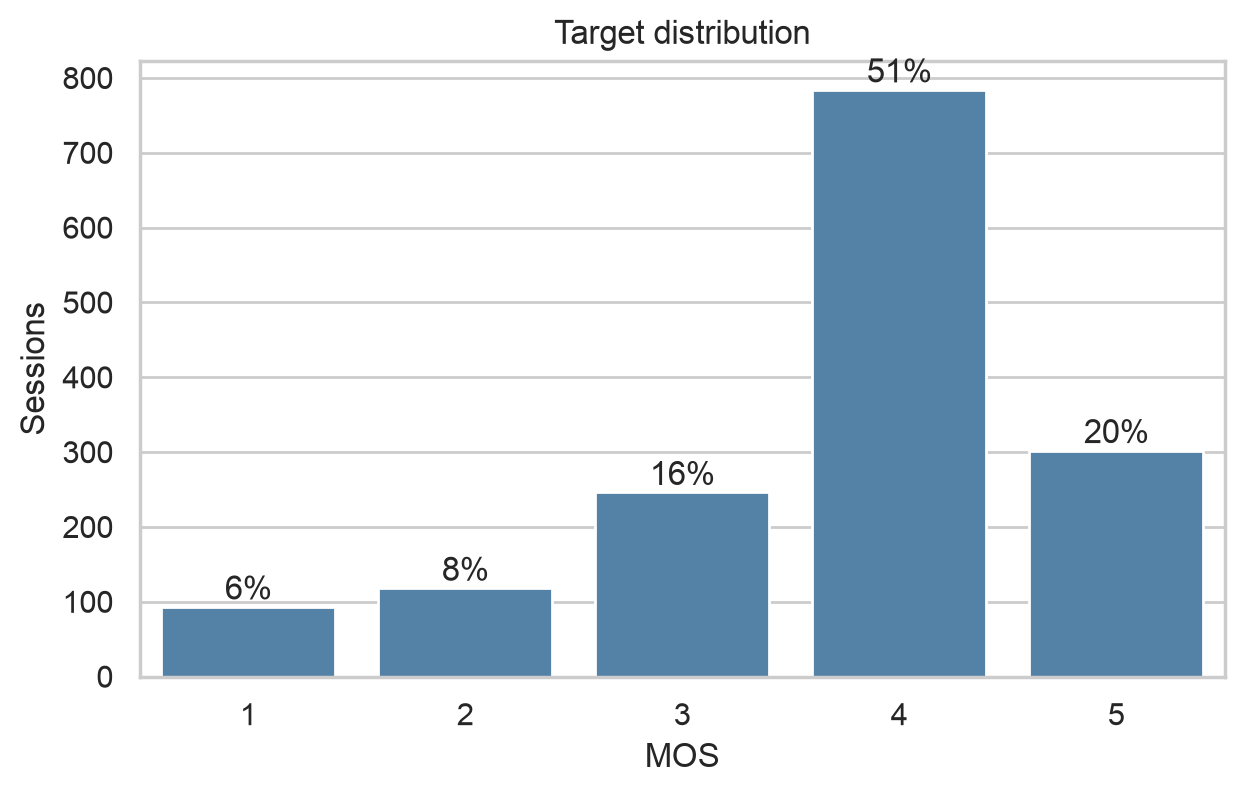
\includegraphics[width=\linewidth]{mos_distribution}
    \caption{MOS distribution}
  \end{subfigure}\hfill
  \begin{subfigure}[b]{0.50\linewidth}
    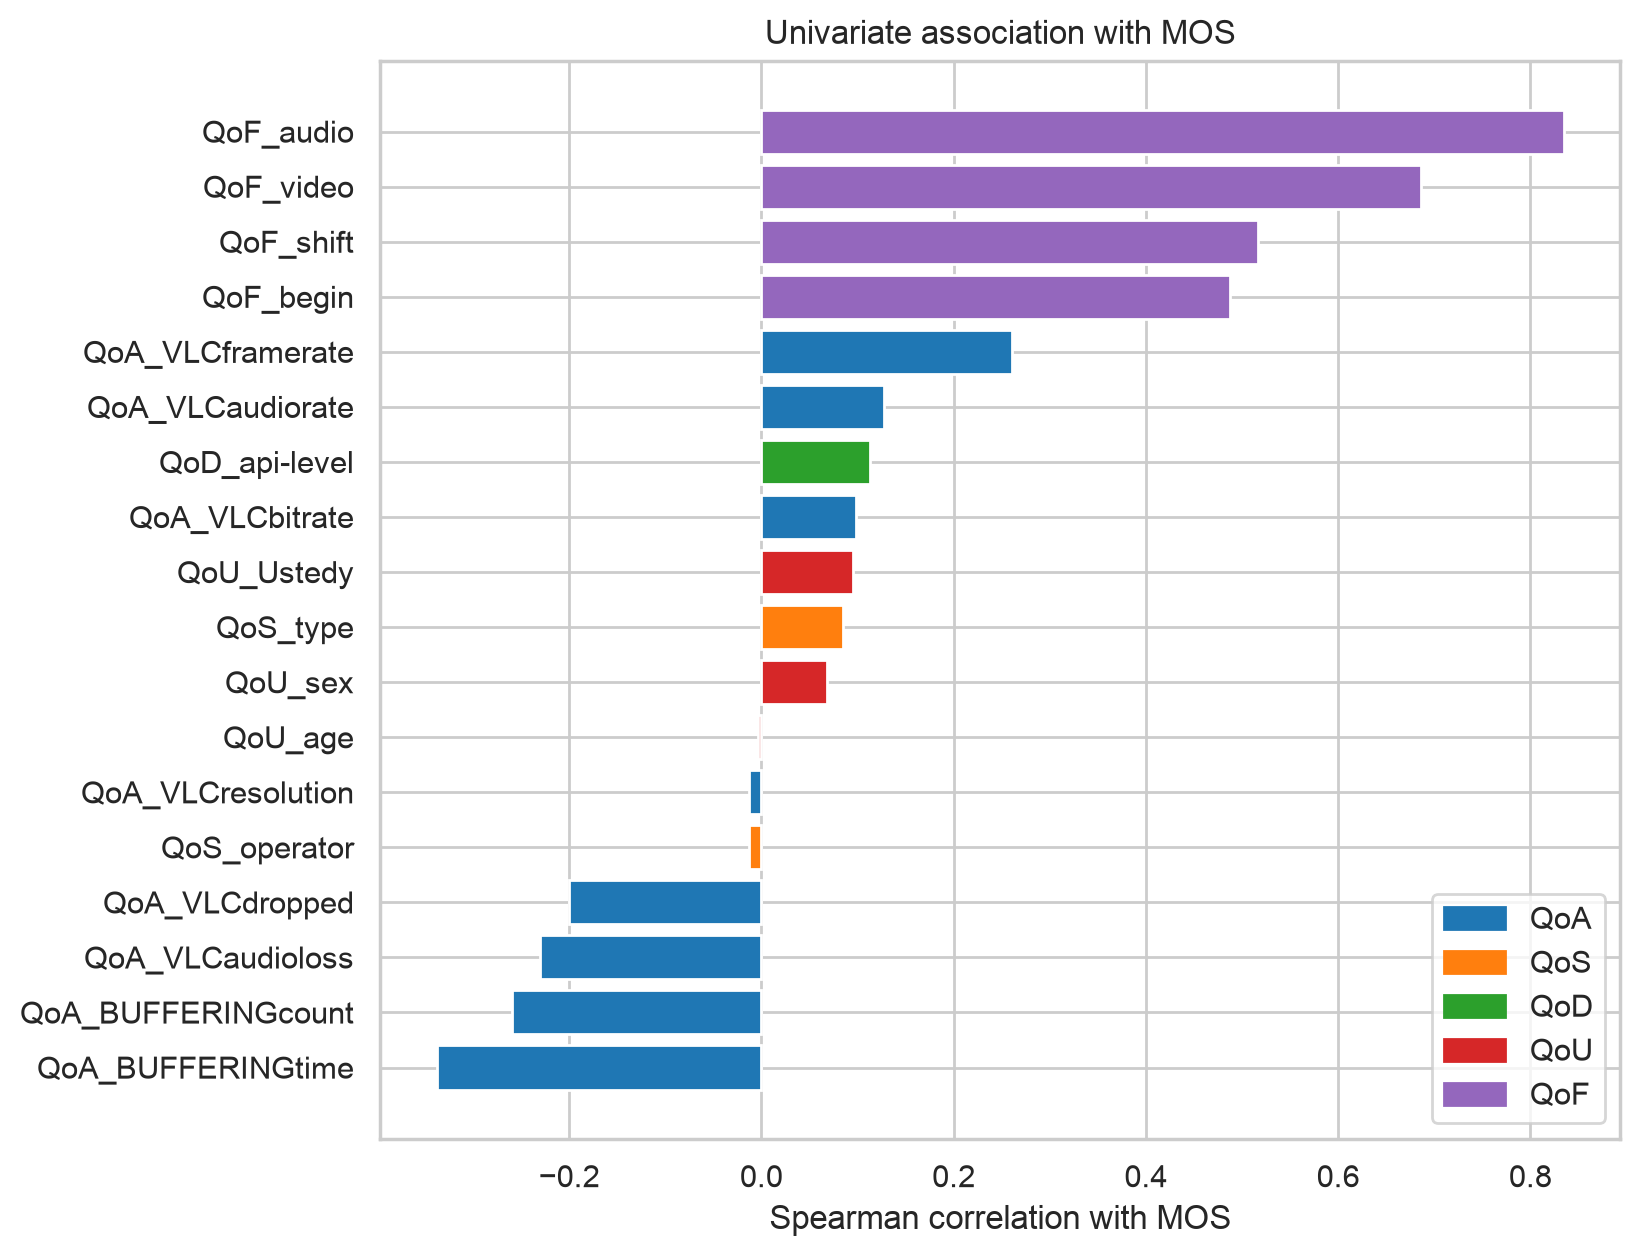
\includegraphics[width=\linewidth]{spearman_with_mos}
    \caption{Spearman correlation with MOS, by factor group}
  \end{subfigure}\\[4pt]
  \begin{subfigure}[b]{0.80\linewidth}
    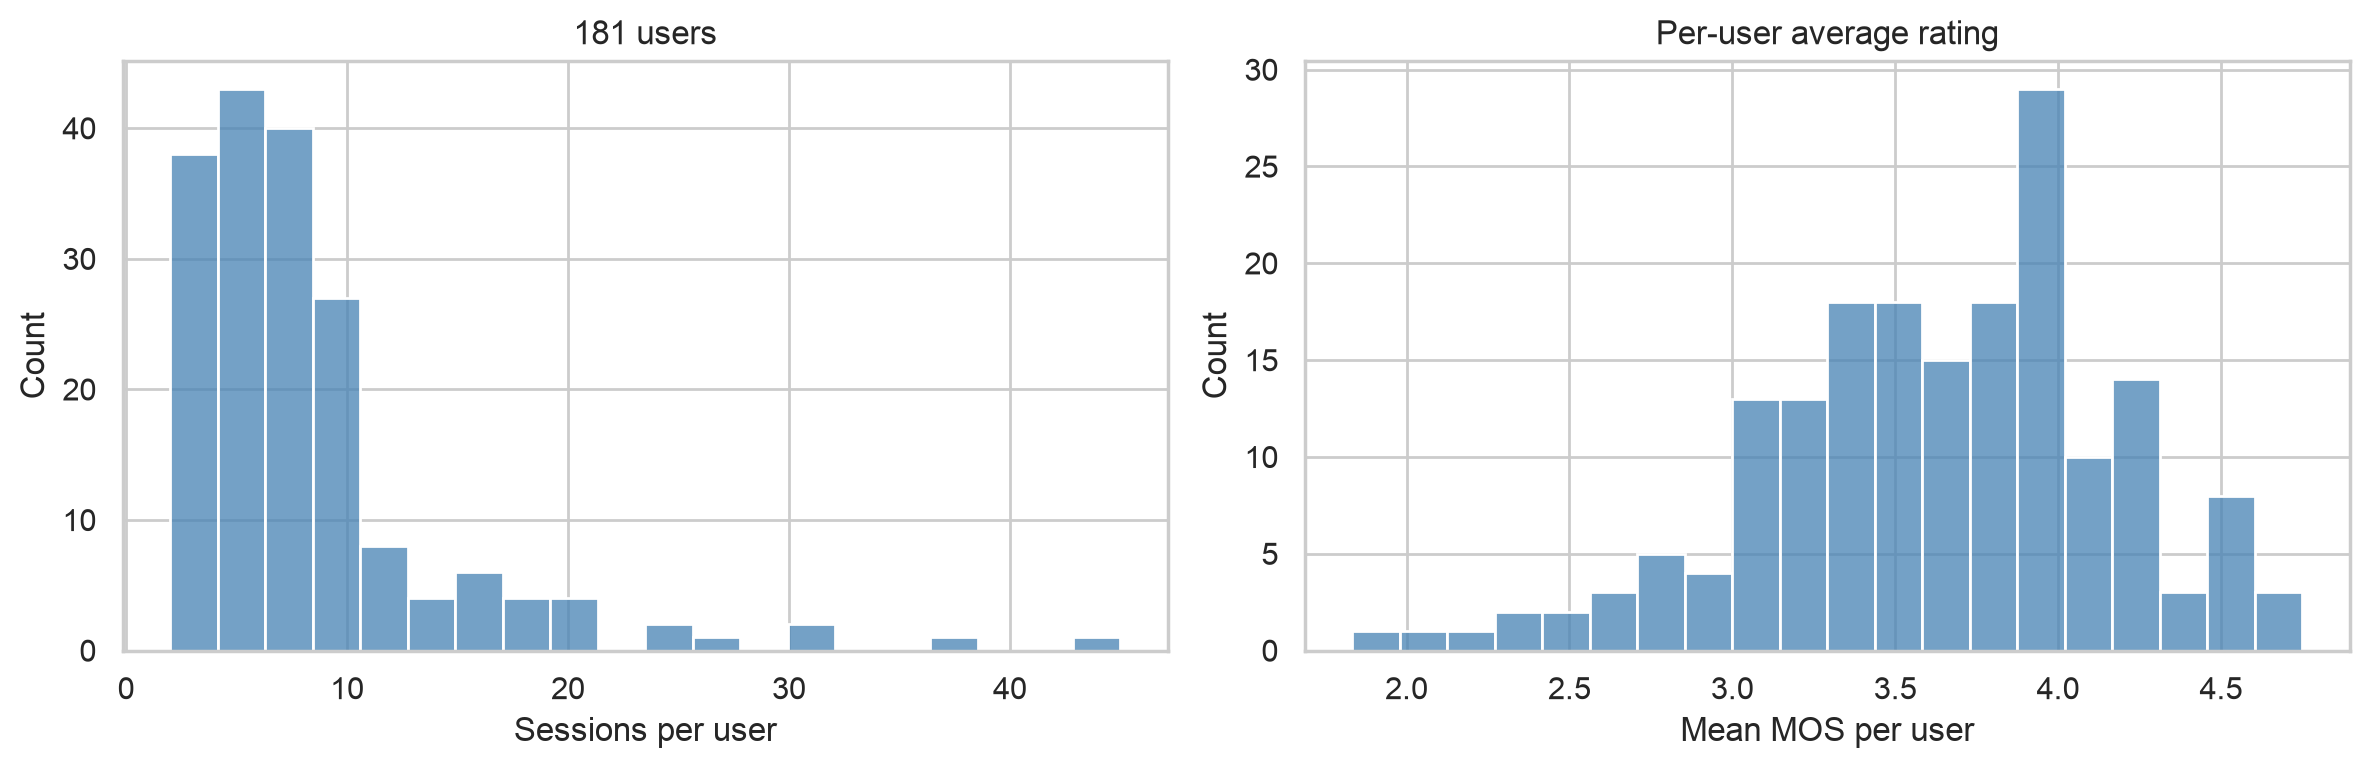
\includegraphics[width=\linewidth]{user_structure}
    \caption{Sessions per tester and per-tester average MOS}
  \end{subfigure}
  \caption{Main findings of the exploratory analysis.}
  \label{fig:eda}
\end{figure}

%=====================================================================
\section{Methods}
%=====================================================================
\paragraph{Preprocessing.}
\code{id} is dropped. \code{user\_id} is used only to group the folds, never as a feature. The target is
recoded to 0--4, which XGBoost requires, and shifted back for reporting. Each model is a scikit-learn
\citep{pedregosa2011sklearn} \code{Pipeline} that applies, in order: $\log(1+x)$ and standardisation to the
four skewed columns, standardisation to the other numeric columns, and one-hot encoding (unknown categories
ignored) to the three nominal columns. The pipeline is fitted inside each cross-validation fold, so no
statistic of the validation fold leaks into training. In the first draft the scaler was fitted outside the
cross-validation.

\paragraph{Models.}
We compare two families with different inductive biases, plus a reference:
\begin{itemize}
  \item \textbf{Dummy} (most frequent class): the floor that any useful model must beat.
  \item \textbf{$k$-nearest neighbours} \citep{cover1967knn}: predicts from similar sessions; simple and
        non-parametric, but sensitive to feature scaling and irrelevant dimensions.
  \item \textbf{Support vector classifier} \citep{cortes1995svm}: a linear kernel tests whether MOS is
        roughly linear in the features; an RBF kernel allows smooth non-linear boundaries.
  \item \textbf{Decision tree} \citep{breiman1984cart}: interpretable thresholds (``more than $x$
        seconds of buffering''), invariant to monotone transformations, but high variance.
  \item \textbf{XGBoost} \citep{chen2016xgboost}: gradient-boosted shallow trees, typically the strongest
        choice for small tabular datasets; it reduces the variance of single trees.
\end{itemize}
Table~\ref{tab:grids} lists the hyperparameter grids, chosen to span under- to over-fitting regimes for
each model (104 configurations in total).

\begin{table}[ht]
  \centering\small
  \caption{Hyperparameter grids explored with \code{GridSearchCV}.}
  \label{tab:grids}
  \begin{tabular}{lp{11.5cm}r}
    \toprule
    Model & Grid & \# configs \\
    \midrule
    kNN & \code{n\_neighbors} $\in\{3,5,7,9,11,15,21\}$, \code{weights} $\in$ \{uniform, distance\} & 14 \\
    SVC & linear: $C\in\{0.1,1,10,100\}$; RBF: $C\in\{0.1,1,10,100\}$, $\gamma\in$ \{scale, 0.01, 0.1\} & 16 \\
    Decision tree & \code{max\_depth} $\in\{3,5,7,10,\text{None}\}$, \code{min\_samples\_leaf} $\in\{1,5,10,20\}$ & 20 \\
    XGBoost & \code{max\_depth} $\in\{2,3,5\}$, \code{learning\_rate} $\in\{0.05,0.1,0.2\}$,
              \code{n\_estimators} $\in\{50,100,200\}$, \code{subsample} $\in\{0.8,1.0\}$ & 54 \\
    \bottomrule
  \end{tabular}
\end{table}

%=====================================================================
\section{Experimental protocol}
\label{sec:protocol}
%=====================================================================
\begin{itemize}
  \item \textbf{Test split.} \code{StratifiedGroupKFold} with 5 folds (seed 42) splits the testers; the
        first fold is held out as test set: 304 sessions from 33 testers, against 1{,}239 sessions from 148
        testers for training. No tester appears in both, and the class proportions of the two sets differ
        by less than 0.3 percentage points.
  \item \textbf{Model selection.} For each model and feature set, \code{GridSearchCV} evaluates every
        configuration with 5-fold \code{StratifiedGroupKFold} on the training testers and keeps the
        configuration with the best mean macro-F1. That configuration is refitted on all training testers.
  \item \textbf{Choice of the final model.} Per feature set, the model with the best cross-validated
        macro-F1 is selected. The test set is used \emph{once}, after this selection. Test scores of the
        other models are reported for transparency only.
  \item \textbf{Metrics.} Macro-F1 (selection), accuracy, and MAE in MOS points.
\end{itemize}
\noindent
Our first draft used a single random 60/20/20 split with selection on the validation set. We replaced it
for three reasons. Cross-validation uses the 20\% formerly reserved for validation as training data, which
matters with 1{,}543 sessions. A single small validation set gives a noisy model ranking. And a random
split mixes the sessions of each tester across sets, which does not reflect predicting QoE for new users.

%=====================================================================
\section{Results}
%=====================================================================
\subsection{Model comparison}
Table~\ref{tab:results} and Figure~\ref{fig:cv} summarise the results; Table~\ref{tab:params} gives the
selected hyperparameters.

\begin{table}[ht]
  \centering\small
  \setlength{\tabcolsep}{4pt}
  \caption{Cross-validated (mean $\pm$ std over 5 grouped folds) and held-out test scores of the best
           configuration of each model. $\star$: model selected on CV macro-F1. MAE is in MOS points
           (lower is better).}
  \label{tab:results}
  \resizebox{\linewidth}{!}{\begin{tabular}{llccc|ccc}
\toprule
 & & \multicolumn{3}{c|}{5-fold grouped CV (training users)} & \multicolumn{3}{c}{Held-out test users} \\
Features & Model & Macro-F1 & Accuracy & MAE & Macro-F1 & Accuracy & MAE \\
\midrule
\multirow{5}{*}{Objective (no QoF)} & Dummy & 0.135 $\pm$ 0.002 & 0.507 $\pm$ 0.010 & 0.690 $\pm$ 0.016 & 0.135 & 0.510 & 0.684 \\
 & kNN & 0.450 $\pm$ 0.020 & 0.520 $\pm$ 0.020 & 0.572 $\pm$ 0.020 & 0.366 & 0.470 & 0.622 \\
 & SVC & 0.431 $\pm$ 0.022 & 0.477 $\pm$ 0.014 & 0.627 $\pm$ 0.024 & 0.358 & 0.434 & 0.704 \\
 & Decision tree & 0.466 $\pm$ 0.033 & 0.531 $\pm$ 0.038 & 0.539 $\pm$ 0.041 & 0.447 & 0.513 & 0.572 \\
 & \textbf{XGBoost}$^\star$ & 0.490 $\pm$ 0.009 & 0.544 $\pm$ 0.030 & 0.531 $\pm$ 0.024 & 0.411 & 0.539 & 0.533 \\
\midrule
\multirow{5}{*}{With feedback (QoF)} & Dummy & 0.135 $\pm$ 0.002 & 0.507 $\pm$ 0.010 & 0.690 $\pm$ 0.016 & 0.135 & 0.510 & 0.684 \\
 & kNN & 0.616 $\pm$ 0.041 & 0.695 $\pm$ 0.016 & 0.328 $\pm$ 0.016 & 0.518 & 0.628 & 0.431 \\
 & SVC & 0.715 $\pm$ 0.047 & 0.778 $\pm$ 0.045 & 0.235 $\pm$ 0.049 & 0.626 & 0.737 & 0.296 \\
 & Decision tree & 0.711 $\pm$ 0.036 & 0.770 $\pm$ 0.043 & 0.250 $\pm$ 0.052 & 0.635 & 0.730 & 0.289 \\
 & \textbf{XGBoost}$^\star$ & 0.774 $\pm$ 0.036 & 0.806 $\pm$ 0.041 & 0.212 $\pm$ 0.055 & 0.689 & 0.753 & 0.266 \\
\bottomrule
\end{tabular}
}
\end{table}

\begin{table}[ht]
  \centering\small
  \caption{Hyperparameters selected by grid search.}
  \label{tab:params}
  \begin{tabular}{lp{0.4\linewidth}p{0.4\linewidth}}
\toprule
Model & Objective (no QoF) & With feedback (QoF) \\
\midrule
kNN & \texttt{n\_neighbors}=5, \texttt{weights}=uniform & \texttt{n\_neighbors}=5, \texttt{weights}=uniform \\
SVC & \texttt{C}=100, \texttt{gamma}=0.1, \texttt{kernel}=rbf & \texttt{C}=0.1, \texttt{kernel}=linear \\
Decision tree & \texttt{max\_depth}=None, \texttt{min\_samples\_leaf}=20 & \texttt{max\_depth}=5, \texttt{min\_samples\_leaf}=10 \\
XGBoost & \texttt{learning\_rate}=0.2, \texttt{max\_depth}=5, \texttt{n\_estimators}=100, \texttt{subsample}=0.8 & \texttt{learning\_rate}=0.05, \texttt{max\_depth}=2, \texttt{n\_estimators}=100, \texttt{subsample}=0.8 \\
\bottomrule
\end{tabular}

\end{table}

\begin{figure}[ht]
  \centering
  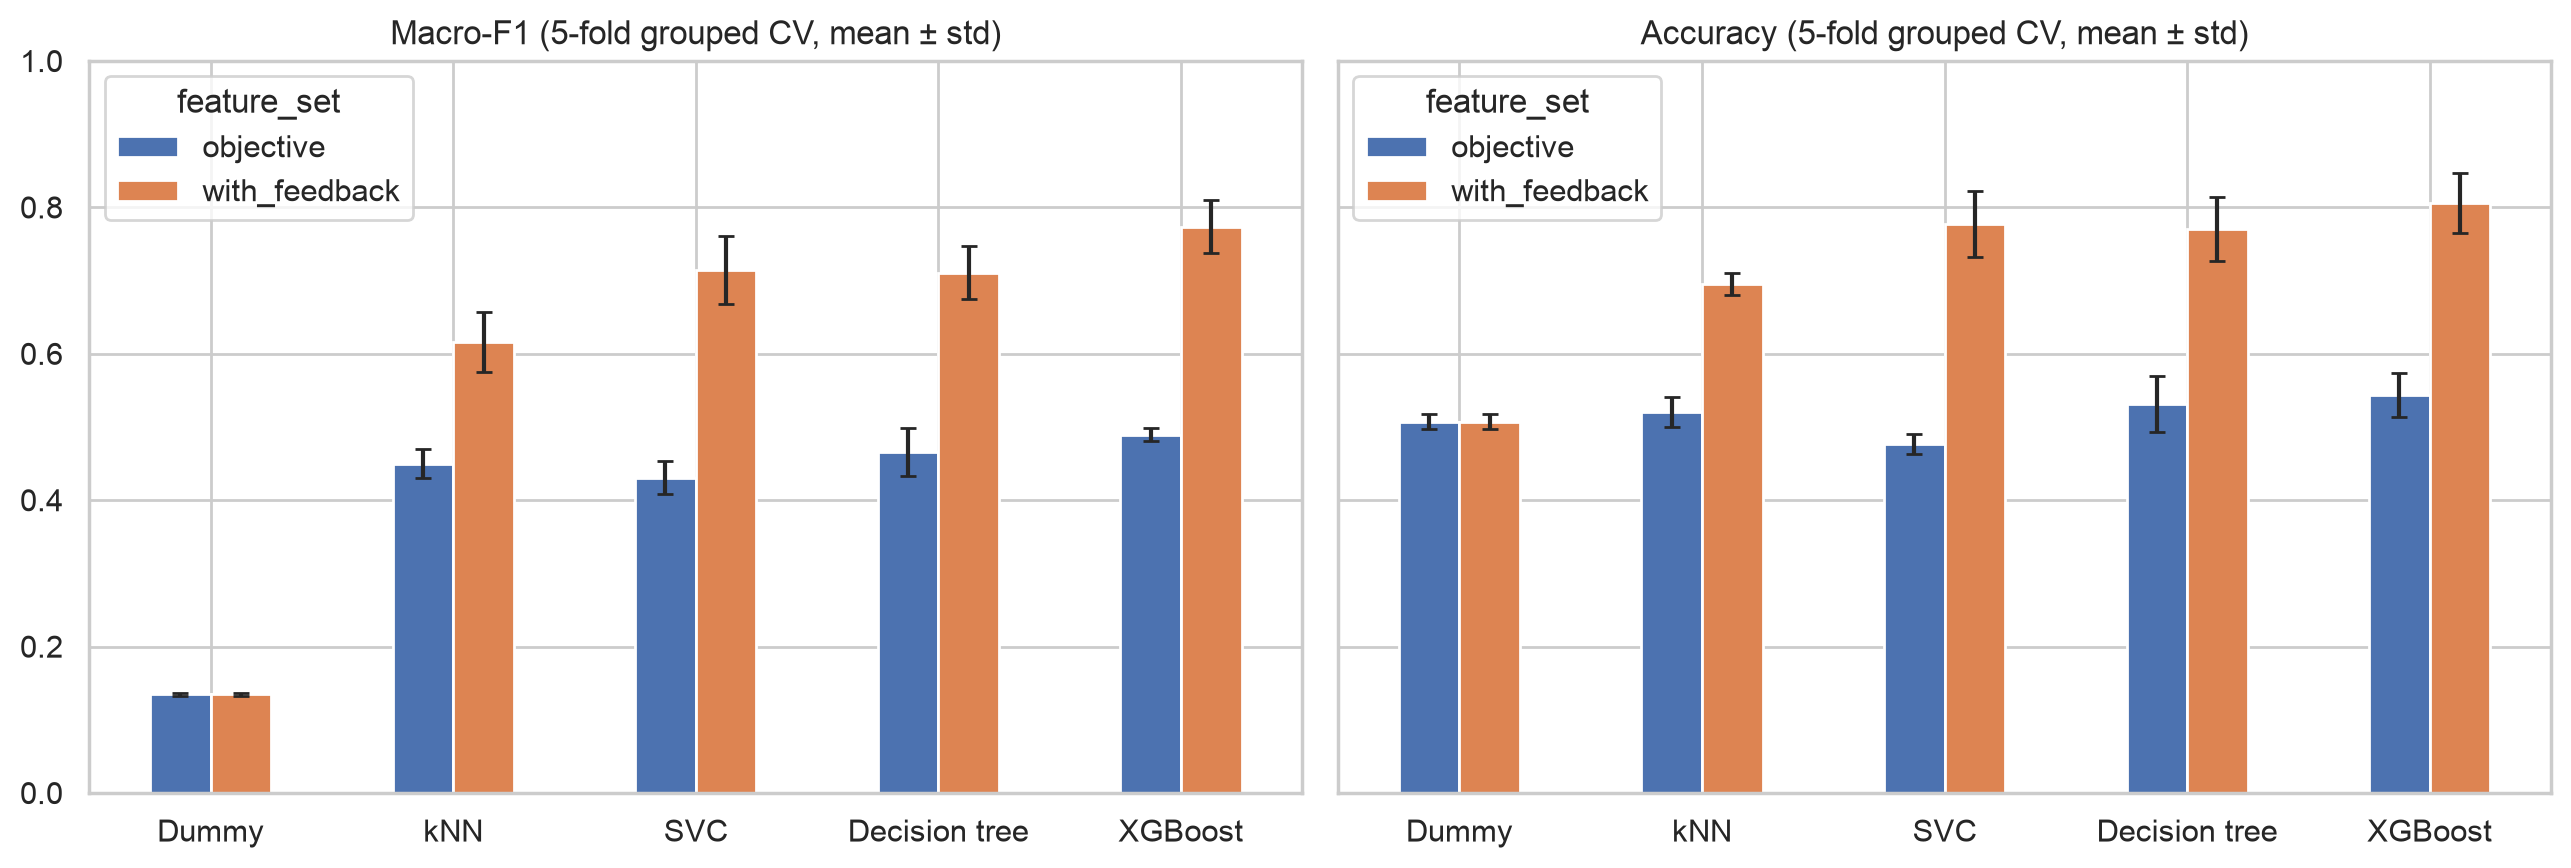
\includegraphics[width=0.95\linewidth]{cv_comparison}
  \caption{Cross-validated macro-F1 and accuracy (mean $\pm$ std over 5 grouped folds) per model and
           feature set.}
  \label{fig:cv}
\end{figure}

\paragraph{Without feedback, MOS is hard to predict.}
On objective features, every model beats the baseline on macro-F1 (0.43--0.49 in CV against 0.13), but
accuracy improves little: XGBoost reaches 0.544 in CV and 0.539 on test users, against 0.51 for the
baseline. MAE falls from 0.68--0.69 to 0.53. The models do learn to recognise clearly bad sessions (MOS 1
recall 0.50 on test), but they cannot separate MOS 4 from MOS 5 (recall 0.80 and 0.17,
Figure~\ref{fig:cm}). Sessions that went well look alike in network and player statistics, and whether a
tester then answers 4 or 5 depends mostly on the tester.

\paragraph{With feedback, performance roughly doubles.}
With QoF ratings, XGBoost reaches 0.774 CV and 0.689 test macro-F1 (accuracy 0.753, MAE 0.27), with
per-class F1 between 0.57 and 0.83. SVC and the decision tree follow closely. kNN is clearly weaker, as
expected for a distance-based method on a mix of one-hot, ordinal and continuous features.

\paragraph{Model ranking.}
XGBoost has the best CV macro-F1 and the lowest MAE in both settings, so it is selected both times. On the
objective test users the decision tree scores higher than XGBoost (0.447 vs 0.411 macro-F1). This
difference is comparable to the largest fold-to-fold standard deviation in CV (0.033), and the test set
holds only 18 sessions of MOS 1 and 23 of MOS 2. We therefore keep the selection made in CV and read the
gap as a reminder of how noisy a single small test set is. In the objective setting, all models except the
decision tree lose 0.07--0.08 macro-F1 between CV and test. The 33 test testers thus appear harder to
predict than the average training fold.

\begin{figure}[ht]
  \centering
  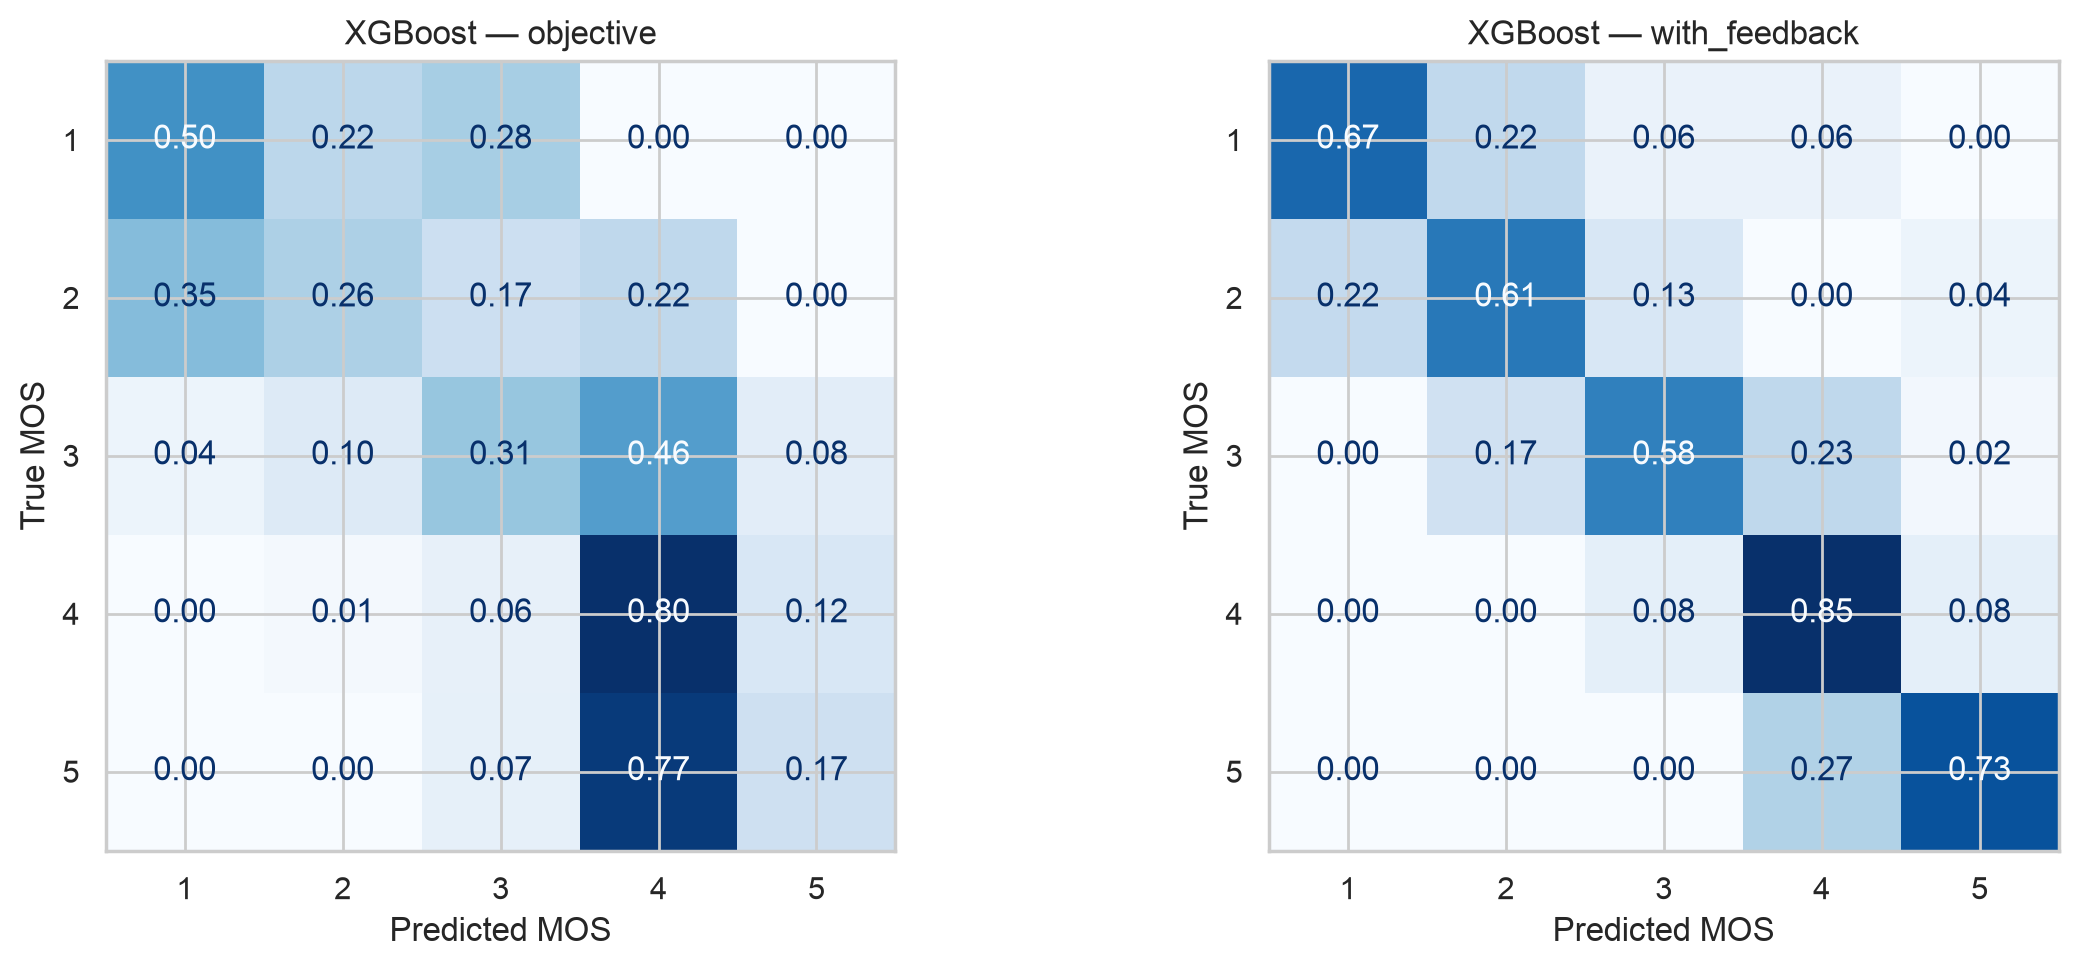
\includegraphics[width=0.82\linewidth]{confusion_matrices}
  \caption{Row-normalised confusion matrices of the selected XGBoost models on the 304 test sessions.}
  \label{fig:cm}
\end{figure}

\subsection{Hyperparameter sensitivity}
Figure~\ref{fig:sens} shows the best CV macro-F1 reached for each value of the main hyperparameters
(objective features).
For kNN, small neighbourhoods work best ($k=5$). Performance declines for larger $k$ (0.45 to 0.37 at
$k=21$), since large neighbourhoods are pulled towards the majority class. Linear SVC is flat around 0.39--0.40, while RBF-SVC
improves monotonically with $C$, showing that the boundary is non-linear and that weak regularisation is
needed. Decision trees improve with depth up to unlimited depth, provided leaves keep at least 20 sessions:
here regularisation by leaf size works better than limiting depth. For XGBoost, a higher learning rate or
more trees help, consistent with a model that underfits at small budgets.
With feedback features the optima move to simpler models (linear SVC with $C=0.1$, depth-2 boosted trees,
Table~\ref{tab:params}), because a few strongly predictive ratings make the problem nearly linear.
Several optima lie on the edge of the grid ($C=100$, \code{learning\_rate}$=0.2$, unlimited depth). These
grids should be extended in further work.

\begin{figure}[ht]
  \centering
  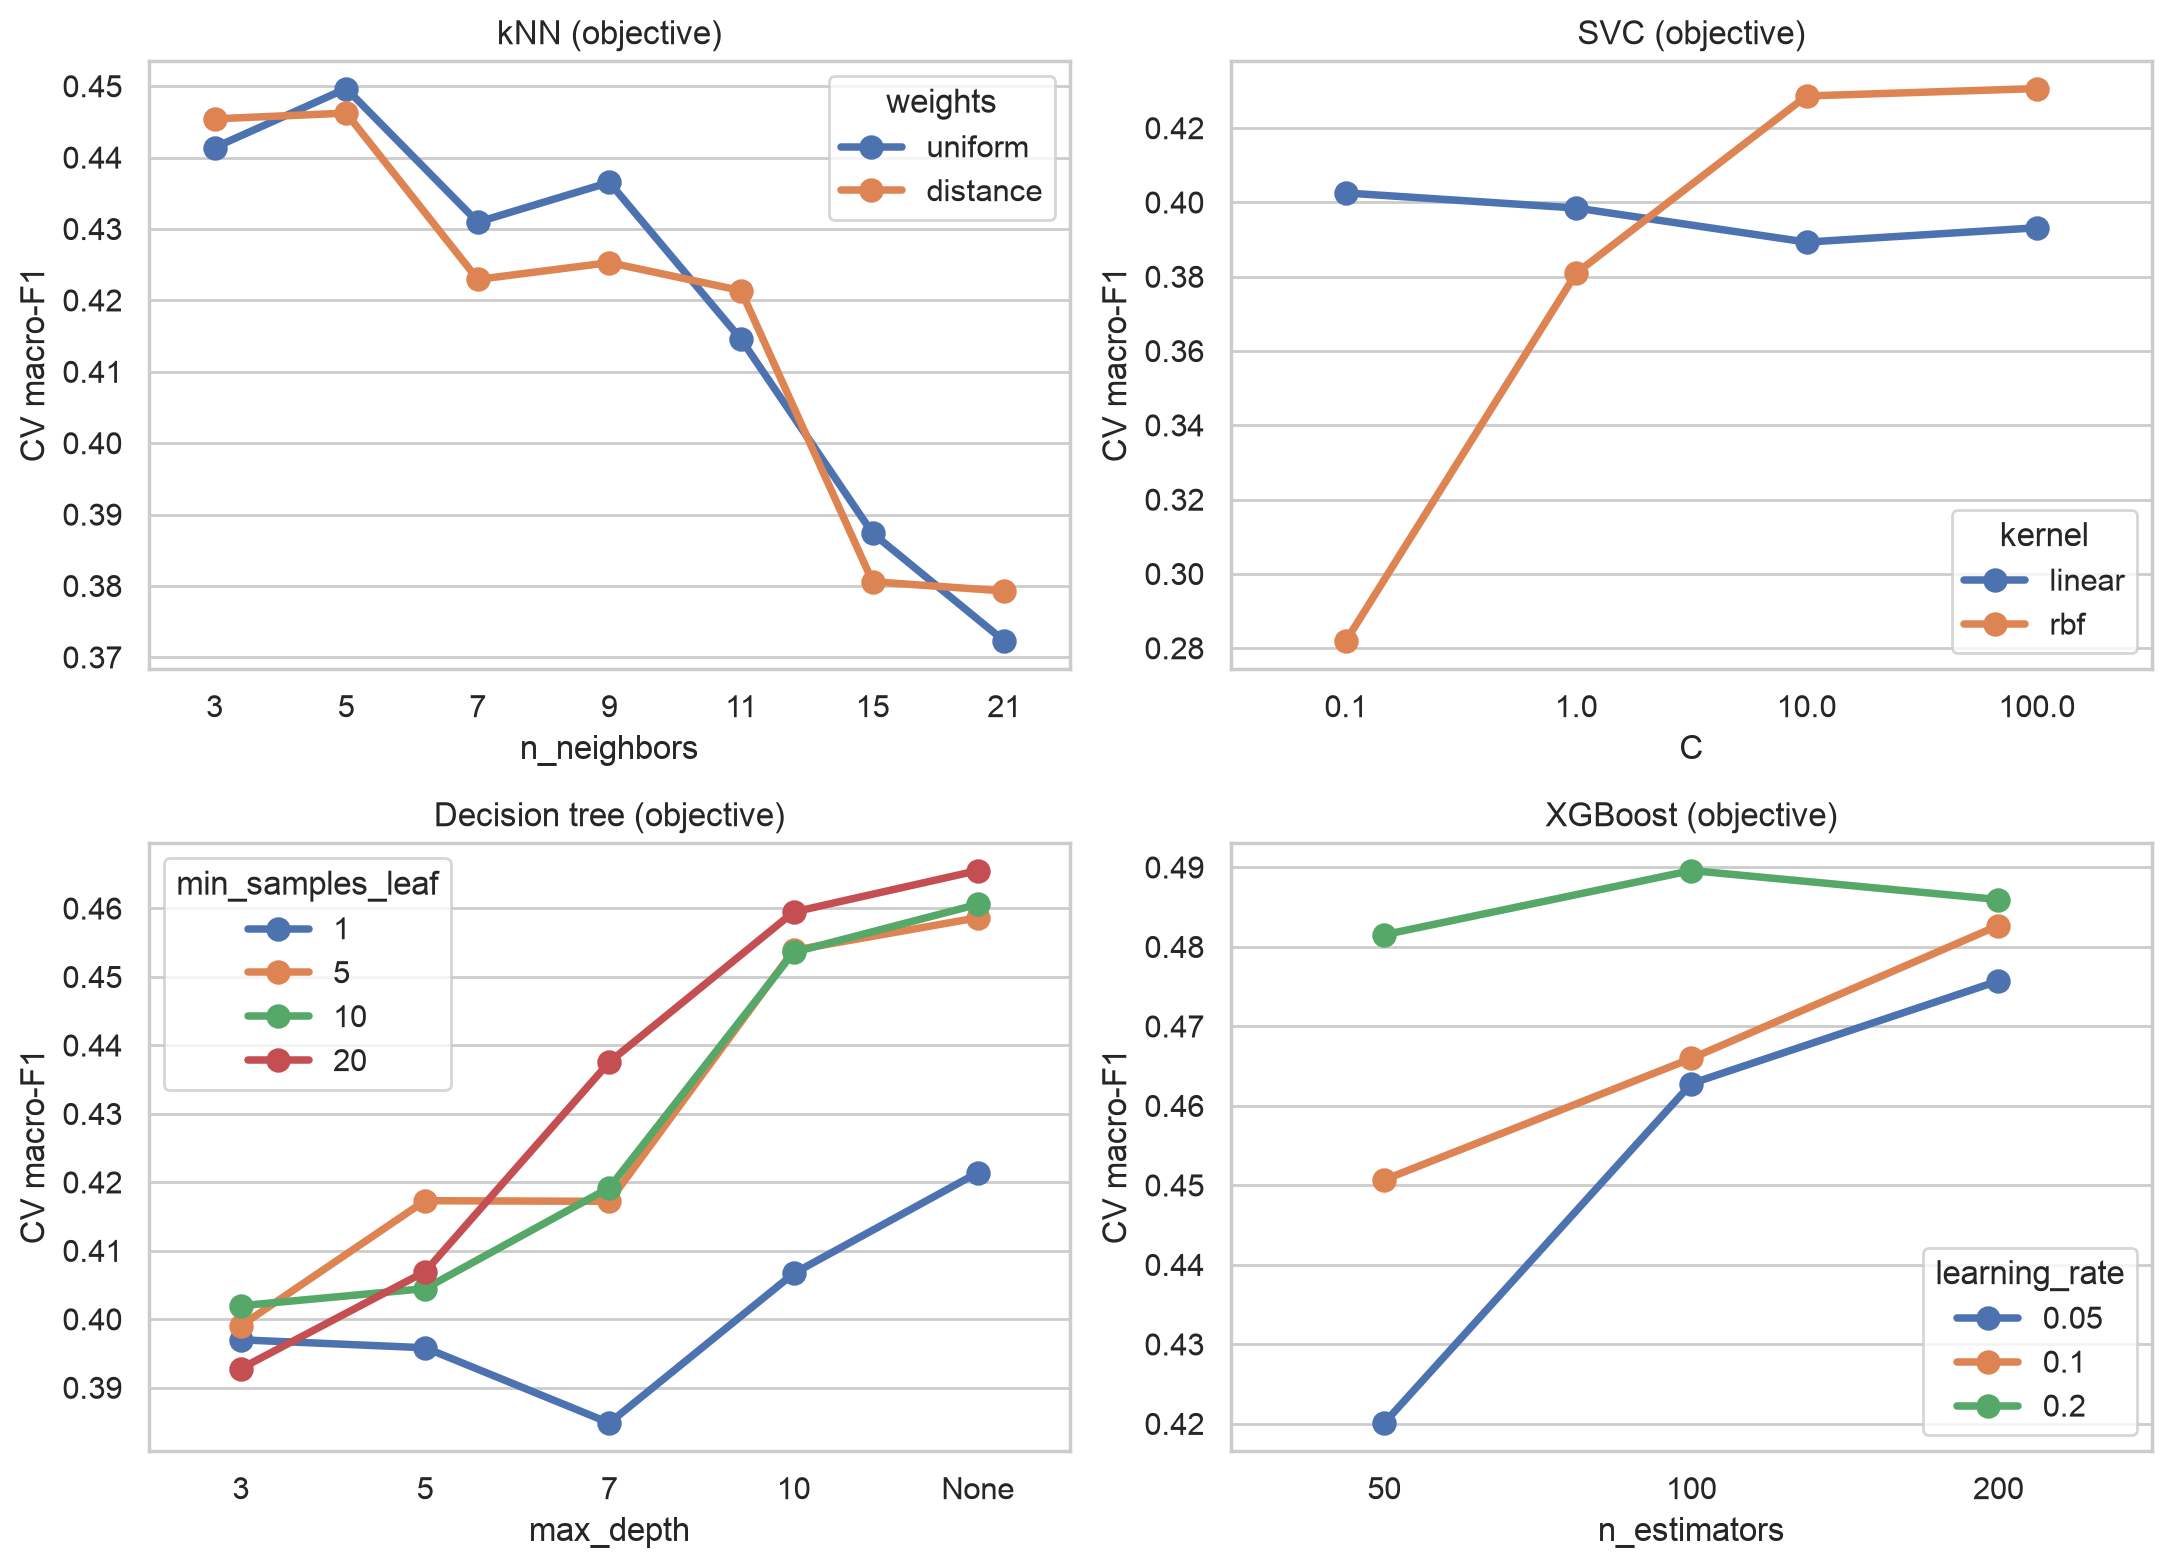
\includegraphics[width=0.78\linewidth]{sensitivity_objective}
  \caption{Hyperparameter sensitivity on objective features: best CV macro-F1 for each value of the
           x-axis parameter and of the hue parameter (maximised over the remaining parameters).}
  \label{fig:sens}
\end{figure}

\subsection{What drives the predictions?}
Figure~\ref{fig:pi} shows permutation importance \citep{breiman2001rf}: the drop in test macro-F1 when one
input column is shuffled (10 repetitions). On objective features, buffering time is by far the most
important input (about 0.16 macro-F1), followed by audio rate, frame rate and bitrate. Network and device
descriptors contribute little, which agrees with the correlation analysis and with the literature on
stalling \citep{hossfeld2012initial,seufert2015survey}. With feedback, \code{QoF\_audio} alone accounts
for a drop of about 0.33 and buffering time remains the most useful measured factor. The model essentially
reproduces how testers aggregate their partial ratings into an overall score.

\begin{figure}[ht]
  \centering
  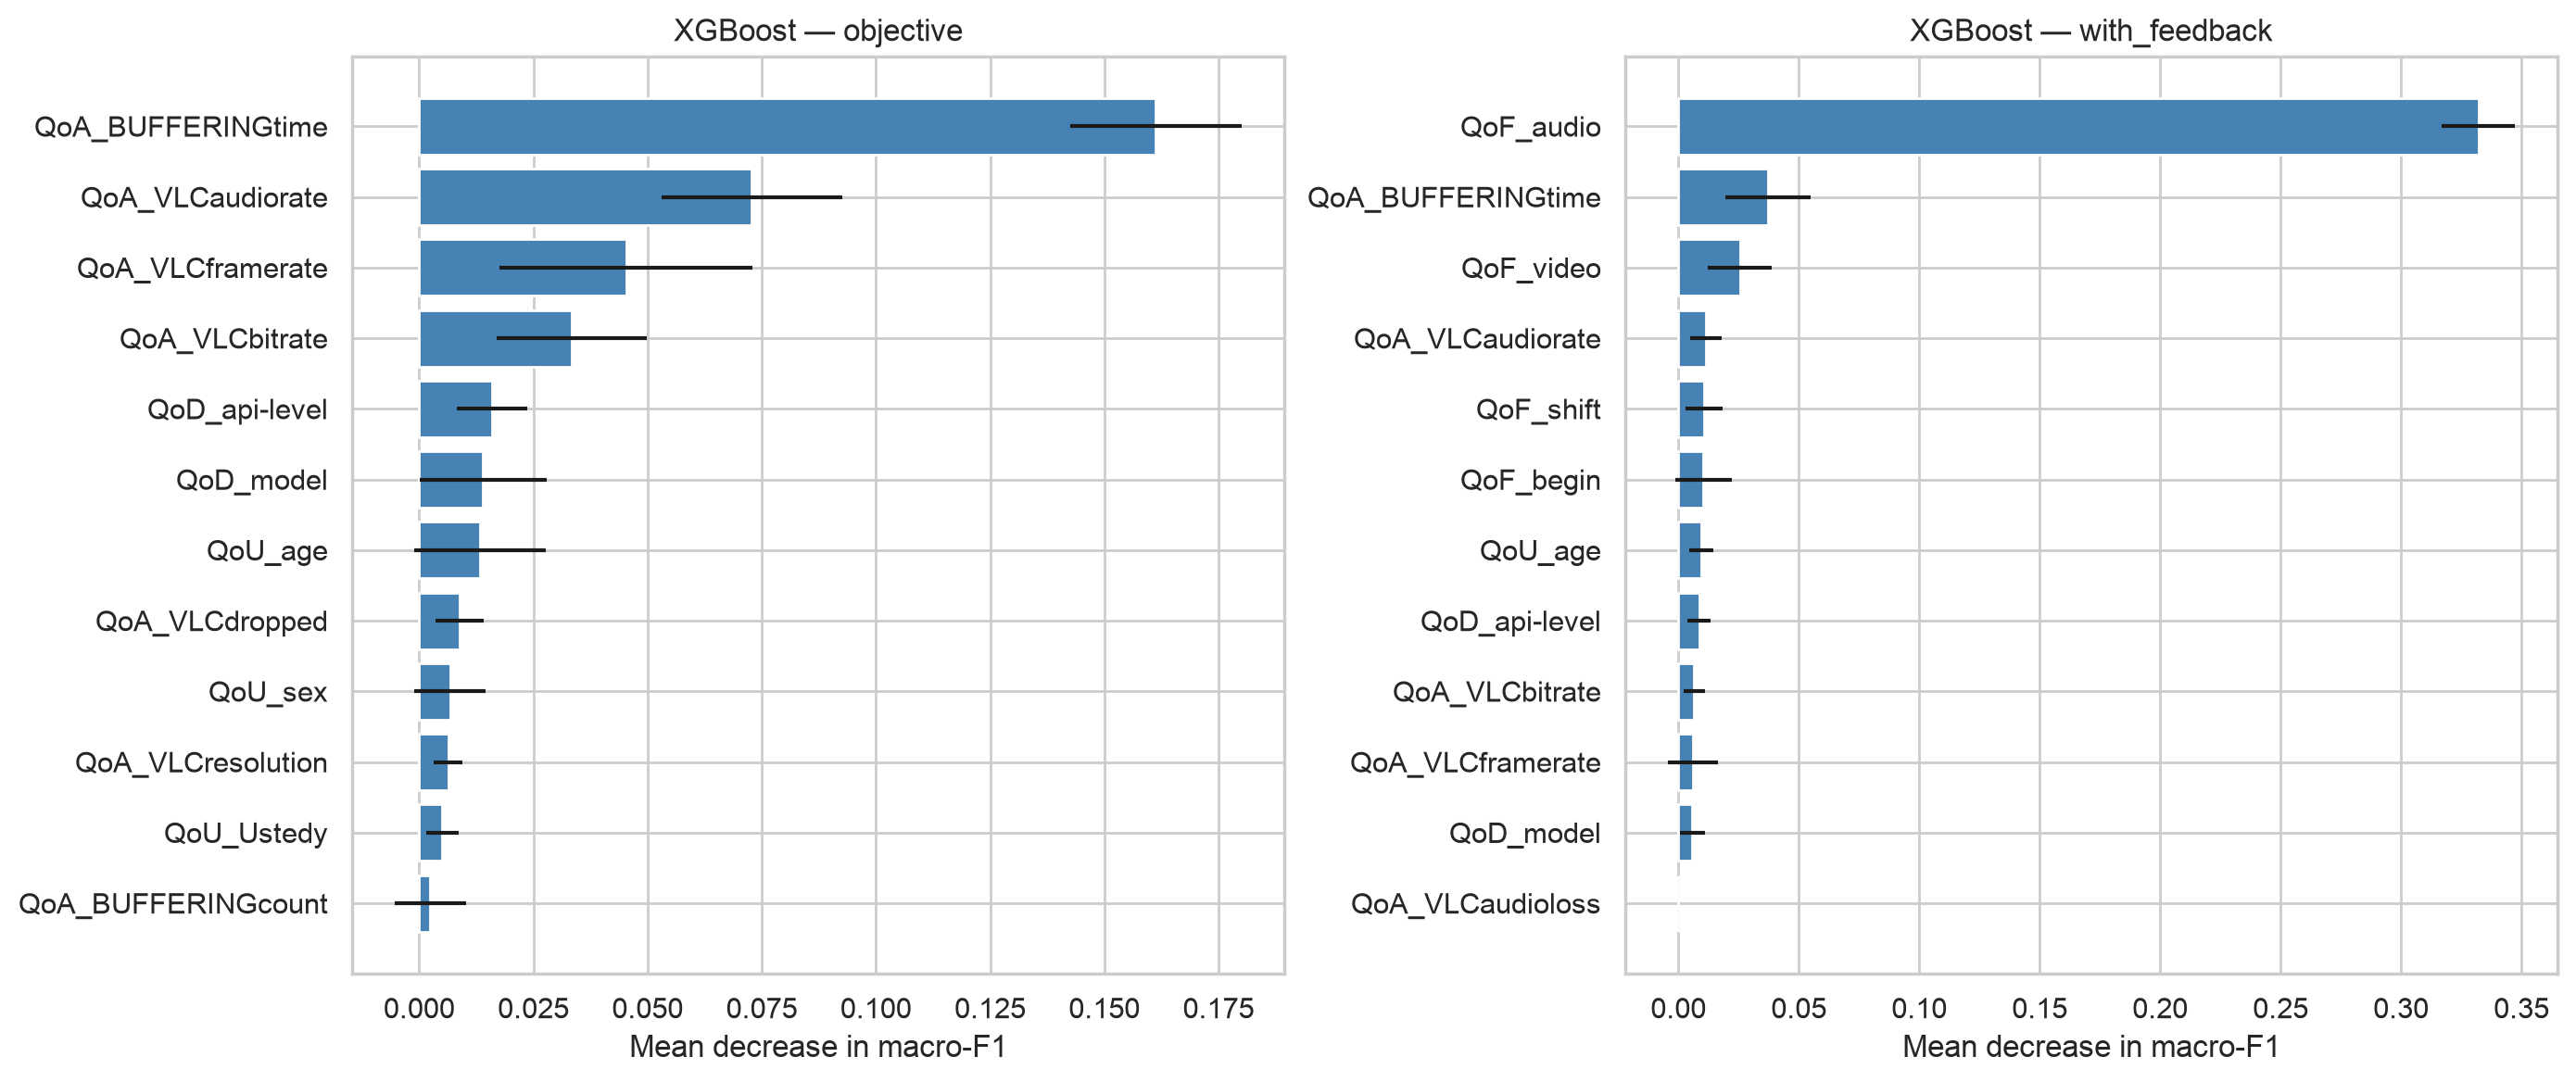
\includegraphics[width=0.95\linewidth]{permutation_importance}
  \caption{Permutation importance of the selected models on test users (mean $\pm$ std over 10
           repetitions; top 12 columns).}
  \label{fig:pi}
\end{figure}

\subsection{Does grouping by user matter?}
\label{sec:split}
To measure the effect of the grouped protocol, we re-evaluated the selected configurations on the training
testers with 5 repetitions of 5-fold CV, once with folds stratified on MOS only (random) and once grouped by
tester (Table~\ref{tab:split}). On objective features, random folds score slightly higher (+0.014
macro-F1, +0.022 accuracy): the direction expected if user overlap inflates performance. The difference is
smaller than one standard deviation, though. With feedback, both schemes give the same result, because the
tester's own ratings already carry the user effect.
Consequently, the drop from 0.80 test accuracy in our first draft (random split, all features) to 0.75 here
is mostly variance between test sets, not user leakage. We keep the grouped split because it matches the
intended use case: predicting QoE for users never seen during training.

\begin{table}[ht]
  \centering\small
  \caption{Random vs.\ user-grouped CV for the selected models (training testers, 5$\times$5-fold CV,
           mean $\pm$ std over 25 folds).}
  \label{tab:split}
  \begin{tabular}{llcc}
\toprule
Features & CV folds & Macro-F1 & Accuracy \\
\midrule
Objective (no QoF) & random & 0.487 $\pm$ 0.034 & 0.564 $\pm$ 0.022 \\
 & grouped & 0.474 $\pm$ 0.046 & 0.542 $\pm$ 0.035 \\
With feedback (QoF) & random & 0.763 $\pm$ 0.036 & 0.803 $\pm$ 0.025 \\
 & grouped & 0.769 $\pm$ 0.041 & 0.805 $\pm$ 0.031 \\
\bottomrule
\end{tabular}

\end{table}

%=====================================================================
\section{Discussion and limitations}
%=====================================================================
\begin{itemize}
  \item \textbf{Small, imbalanced data.} 1{,}543 sessions from 181 testers, and 18--23 test sessions for
        MOS 1 and 2. A single held-out split gives uncertain test scores, as the gap between CV and test and
        the decision-tree/XGBoost inversion show. Nested or repeated grouped CV would give confidence
        intervals for the final estimate.
  \item \textbf{Ordinal target treated as nominal.} The classifiers ignore that 4 is closer to 5 than to 1;
        we only account for it through MAE. Regression or ordinal models would use this structure directly.
  \item \textbf{Feedback features.} The ``with feedback'' results are an upper bound: QoF ratings come from
        the same questionnaire as MOS and are not available when QoE must be estimated passively.
  \item \textbf{User bias.} Testers rate systematically higher or lower (24.5\% of the variance is
        between-user). No model can correct for the personal bias of an unseen user without some feedback
        from that user. This sets a ceiling for objective-only prediction.
  \item \textbf{Class imbalance.} We did not use class weights or resampling, so that all models are
        compared on the same footing (XGBoost has no \code{class\_weight} option and would need explicit
        sample weights). This may limit recall on MOS 2 and MOS 5.
  \item \textbf{External validity.} One campaign around Paris, 9 device types, young and highly educated
        testers, and a VLC-based player. The results may not transfer to other populations, adaptive
        streaming players or current networks.
\end{itemize}

%=====================================================================
\section{Conclusion}
%=====================================================================
On the PoQeMoN dataset, gradient-boosted trees (XGBoost) were the most accurate of the models we compared,
in both settings. The setting matters more than the model, though. With the testers' partial ratings, MOS
is predicted with 0.75 accuracy and an average error of 0.27 MOS points, but most of this comes from one
rating (audio). From quantities a provider can measure, the best models reach only 0.54 accuracy (MAE 0.53),
little above always predicting ``good''. Buffering time is the single most informative measurement, and
distinguishing ``good'' from ``excellent'' is largely a matter of the individual user. Promising next steps
are ordinal models, repeated grouped evaluation, extended grids, and features describing each
user's rating tendency, which a deployed system could estimate from a few ratings.

%=====================================================================
\section*{Reproducibility}
%=====================================================================
All results come from \code{notebooks/poqemon-qoe-project.ipynb}, which downloads the data, runs from top to
bottom without manual steps, and writes the figures and result tables used here (\code{figures/},
\code{results/}). The seed is 42 for the splits, the CV folds, all stochastic models and permutation
importance; the repeated CV of Section~\ref{sec:split} uses seeds 42--46. Two consecutive runs gave
identical result files. Software: Python 3.14.4, NumPy 2.5.4, pandas 3.1.0, scikit-learn 1.9.1,
XGBoost 3.4.1, Matplotlib 3.11.2, seaborn 0.13.2 (pinned in \code{requirements.txt}). Installation and
run instructions are in the repository \code{README.md}.

%=====================================================================
\section*{Contributions}
%=====================================================================
\textbf{Gonzalo} carried out the exploratory data analysis and the tree-based models (decision tree and
XGBoost). \textbf{Salma} prepared the train/validation/test split and implemented the distance-based models
($k$-NN and SVC). Both members analysed and interpreted the results and wrote the report together.

%=====================================================================
\section*{Use of generative AI}
%=====================================================================
We used Claude Code (Anthropic, model Claude Opus 5.5) to restructure our initial notebook into a single
reproducible pipeline, to review the evaluation protocol (preprocessing leakage, encoding of categorical
variables, grouping of sessions by tester, treatment of the feedback columns), and to draft this report from
the notebook outputs.
We checked its output as follows. We re-ran the notebook from scratch twice and obtained identical results.
We checked every number in this report against the generated result files (the tables are produced
directly from them by \code{report/make\_tables.py}). We read and understood all the code, and we verified
claims with additional experiments where they were doubtful: the effect of the grouped split
(Section~\ref{sec:split}) was tested after a first explanation turned out to be overstated. We are
responsible for the content of this report.
\todo{Adjust this declaration so it accurately describes your own use of the tool.}

\bibliographystyle{plainnat}
\bibliography{references}

\end{document}
